\documentclass{article}
\usepackage{pgfplots}
\pgfplotsset{compat=newest}

\begin{document}

\begin{figure}[h]
    \centering
    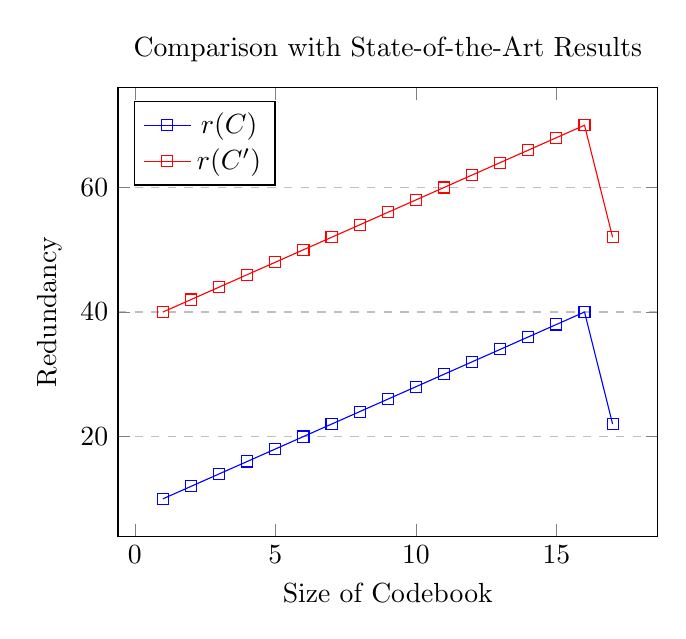
\begin{tikzpicture}
        \begin{axis}[
            title={Comparison with State-of-the-Art Results},
            xlabel={Size of Codebook},
            ylabel={Redundancy},
            legend pos=north west,
            ymajorgrids=true,
            grid style=dashed,
        ]
            \addplot[
                color=blue,
                mark=square,
                ]
            coordinates {
                (1,10)(2,12)(3,14)(4,16)(5,18)(6,20)(7,22)(8,24)(9,26)(10,28)(11,30)(12,32)(13,34)(14,36)(15,38)(16,40)(17,22)
            };
            \addplot[
                color=red,
                mark=square,
                ]
            coordinates {
                (1,40)(2,42)(3,44)(4,46)(5,48)(6,50)(7,52)(8,54)(9,56)(10,58)(11,60)(12,62)(13,64)(14,66)(15,68)(16,70)(17,52)
            };
            \legend{$r(C)$, $r(C')$}
        \end{axis}
    \end{tikzpicture}
    \caption{Comparison graph with state-of-the-art results \cite{Smagloy_Welter_Wachter-Zeh_Yaakobi_2020}. Our approach computes three times for different codebook sizes and returns the length of the sequence $n$. The state-of-the-art result is given by the formula $10\log(n) + 3\log(q) + 11$, where $q=4$.}
    \label{fig:comparison}
\end{figure}

\end{document}